%\documentclass[tikz]{standalone}
\documentclass[aspectratio=169]{beamer}
\beamertemplatenavigationsymbolsempty
%\documentclass{beamer}
\usepackage{tikz}
\usetikzlibrary{arrows}
\usetikzlibrary{positioning}
%for animation
\tikzset{
  invisible/.style={opacity=0},
  visible on/.style={alt={#1{}{invisible}}},
  alt/.code args={<#1>#2#3}{%
    \alt<#1>{\pgfkeysalso{#2}}{\pgfkeysalso{#3}} % \pgfkeysalso doesn't change the path
  },
}

\tikzstyle{node} = [rectangle, thick, draw =black!80]
\tikzstyle{nodeu} = [rectangle, thick, draw =black!80, fill=gray!20]
\tikzstyle{nodei} = [rectangle, double, draw =black!80]

\begin{document}

%\input{scm0.tikz}

\begin{frame}

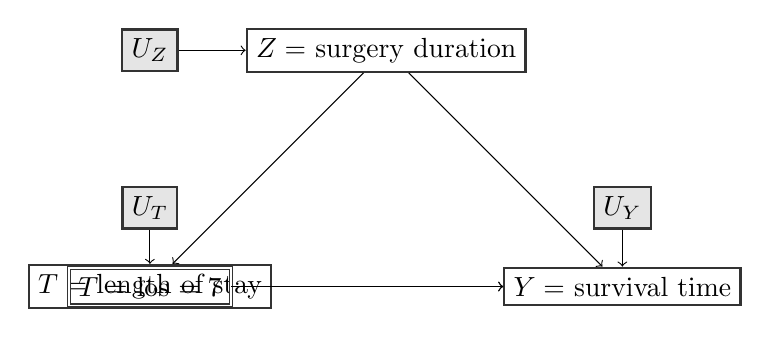
\begin{tikzpicture}
 \node[nodeu, visible on=<1-4>] (uz) at (-3, 3) {$U_Z$};
 \node[node, visible on=<1-5>] (z) at (0, 3) {$Z=$ surgery duration};
 \node[nodeu, visible on=<2-4>] (ut) at (-3, 1) {$U_T$};
 \node[node, visible on=<2-3>] (t) at (-3, 0) {$T=$ length of stay};
 \node[nodei, visible on=<4->] (ti) at (-3, 0) {$T=$ los $=7$};
 \node[nodeu, visible on=<3-4>] (uy) at (3, 1) {$U_Y$};
 \node[node, visible on=<3->] (y) at (3, 0) {$Y=$ survival time};

 % Edges
 \draw[->, visible on=<1-4>] (uz) -- (z);
 \draw[->, visible on=<2-3>] (ut) -- (t);
 \draw[->, visible on=<3-4>] (uy) -- (y);

 \draw[->, visible on=<2-3>] (z) -- (t);
 \draw[->, visible on=<3->] (z) -- (y);
 \draw[->, visible on=<3>] (t) -- (y);
 \draw[->, visible on=<4->] (ti) -- (y);

\end{tikzpicture}

\end{frame}

\end{document}
